\documentclass[a4paper]{article}

%% Language and font encodings
\usepackage[english]{babel}
\usepackage[utf8x]{inputenc}
\usepackage[T1]{fontenc}
\usepackage{hyperref}

%% Sets page size and margins
\usepackage[a4paper,top=3cm,bottom=2cm,left=3cm,right=3cm,marginparwidth=1.75cm]{geometry}

%% Useful packages
\usepackage{amsmath}
\usepackage{graphicx}
\usepackage{url}
\usepackage{listings}
\usepackage{enumitem}

%% Solidity highlighting for listings
% Copyright 2017 Sergei Tikhomirov, MIT License
% https://github.com/s-tikhomirov/solidity-latex-highlighting/

\usepackage{listings, xcolor}

\definecolor{verylightgray}{rgb}{.97,.97,.97}

\lstdefinelanguage{Solidity}{
	keywords=[1]{anonymous, assembly, assert, balance, break, call, callcode, case, catch, class, constant, continue, contract, debugger, default, delegatecall, delete, do, else, event, export, external, false, finally, for, function, gas, if, implements, import, in, indexed, instanceof, interface, internal, is, length, library, log0, log1, log2, log3, log4, memory, modifier, new, payable, pragma, private, protected, public, pure, push, require, return, returns, revert, selfdestruct, send, storage, struct, suicide, super, switch, then, this, throw, transfer, true, try, typeof, using, value, view, while, with, addmod, ecrecover, keccak256, mulmod, ripemd160, sha256, sha3}, % generic keywords including crypto operations
	keywordstyle=[1]\color{blue}\bfseries,
	keywords=[2]{address, bool, byte, bytes, bytes1, bytes2, bytes3, bytes4, bytes5, bytes6, bytes7, bytes8, bytes9, bytes10, bytes11, bytes12, bytes13, bytes14, bytes15, bytes16, bytes17, bytes18, bytes19, bytes20, bytes21, bytes22, bytes23, bytes24, bytes25, bytes26, bytes27, bytes28, bytes29, bytes30, bytes31, bytes32, enum, int, int8, int16, int24, int32, int40, int48, int56, int64, int72, int80, int88, int96, int104, int112, int120, int128, int136, int144, int152, int160, int168, int176, int184, int192, int200, int208, int216, int224, int232, int240, int248, int256, mapping, string, uint, uint8, uint16, uint24, uint32, uint40, uint48, uint56, uint64, uint72, uint80, uint88, uint96, uint104, uint112, uint120, uint128, uint136, uint144, uint152, uint160, uint168, uint176, uint184, uint192, uint200, uint208, uint216, uint224, uint232, uint240, uint248, uint256, var, void, ether, finney, szabo, wei, days, hours, minutes, seconds, weeks, years},	% types; money and time units
	keywordstyle=[2]\color{teal}\bfseries,
	keywords=[3]{block, blockhash, coinbase, difficulty, gaslimit, number, timestamp, msg, data, gas, sender, sig, value, now, tx, gasprice, origin},	% environment variables
	keywordstyle=[3]\color{violet}\bfseries,
	identifierstyle=\color{black},
	sensitive=false,
	comment=[l]{//},
	morecomment=[s]{/*}{*/},
	commentstyle=\color{gray}\ttfamily,
	stringstyle=\color{red}\ttfamily,
	morestring=[b]',
	morestring=[b]"
}

\lstset{
	language=Solidity,
	backgroundcolor=\color{verylightgray},
	extendedchars=true,
	basicstyle=\footnotesize\ttfamily,
	showstringspaces=false,
	showspaces=false,
	numbers=left,
	numberstyle=\footnotesize,
	numbersep=9pt,
	tabsize=2,
	breaklines=true,
	showtabs=false,
	captionpos=b
}
\lstset{escapeinside={<@}{@>}}


\title{Runtime Verification of Smart Contracts \\
\large On the Ethereum network \\}

\author{Lars Stegeman [s1346466]\\ l.stegeman@student.utwente.nl}

\begin{document}

\maketitle

\tableofcontents



\section{Abstract}

\section{Introduction}

\section{Solidity}
Section explains basics of solidity in order to understand the rest of the paper. Same section as in ResearchTopics

\section{Tool Overview}
\begin{itemize}
  \item Tool works in two phases validation and generation.
  \item Validation typechecks and checks if annotations are well formed according to grammar.
  \item Generation generates original solidity code with extra added code to check annotations at runtime.
  \item Approach uses a Solidity grammar that can be updated easily for future updates.
  \item Output of validation phase can be used for other verification tools (result is a parse tree).
  \item Annotations can be defined as invariants and pre or post conditions for functions.
  \item Annotations use JML like syntax.
  \item Tool can be used both during development (as extra test cases) or on the actual live blockchain (this probably costs a lot of extra gas = ether).
\end{itemize}
\begin{center}
  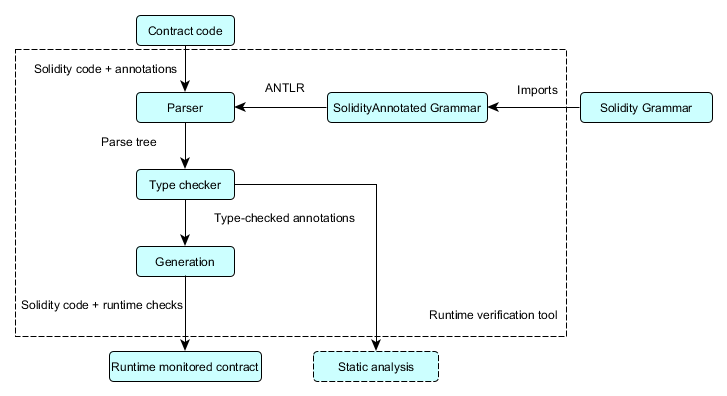
\includegraphics[width=\textwidth,height=\textheight,keepaspectratio]{resources/ToolOverview.png}
\end{center}
In the picture the complete overview of the tool can be seen. Within the dashed square the implemented parts are visible. The arrows indicate the flow of the contract code throughout the program. \\
First contract code has to be annotated according to a specified grammar. Section \ref{sec:annotationlanguage} explains the grammar in more detail and gives some example annotations. The tool ANTLR is used to generate code for the lexer and parser. The result of this step is a parse tree which can be used for later stages. \\
The next step is type checking the annotations. This uses the parse tree to examine the annotations and check if they are valid. The type checking is done bottom up and works in two phases. The first phase collects all the relevant variables. This includes state variables and function definitions (function name, arguments and return values). The next phase uses this information to do the actual type checking of the annotations. This is explained in more detail in Section \ref{sec:typechecker}. \\
The result of the type checker phase are type-checked annotations. In practice these are parse tree objects in which the types correspond to the operators used and the identifiers that are used are also defined in the contract. This is used as input for the generation phase. The generation phase will operate on the information that is created during the type checker phase. For each annotation it will generate the code that is needed to check it during runtime. This happens in a single passage of the complete parse tree. Details on this phase can be found in Section \ref{sec:generation}. \\
Using the annotation grammar all specifications can be expressed. But not all specifications can be translated to code that can be checked at runtime. This means that some annotations will not be translated to runtime monitored contract code. This is the case because of limitations within the Solidity language. For example the mapping type is not iterable and the keys are not known. This means that mappings have to be replaced with other constructions. In the current state of the tool only basic mappings can be replaced with iterable constructions. \\
The output of the type checker phase can also be used for other static analysis tools. The benefit of using the tool to validate the annotations is that the result is a type checked parse tree that can be parsed and traversed in various ways to be useful for static verification methods. 

\section{Annotation Language}
\label{sec:annotationlanguage}
The first step towards implementing the tool is to define an annotation syntax, and formally write this down using a grammar. The parser generator that is used is called ANTLR. Using the grammar definition the lexer and parser will be automatically generated. The output of this phase is a parse tree that can be used in later stages of the tool.

\subsection{Grammar definition}
There already exists a grammar for the complete Solidity language. This grammar is written down using the language that is used by ANTLR tool. ANTLR has the capabilities to extend certain grammars. This is done by inheritance over the original grammar. This principle is explained in detail here (find ref). We will use this principle to extend the grammar of Solidity to recognize the special annotations that will later be used in the tool. \\
The annotations have certain requirements that can be summarized the following way. Later each requirement is discussed in detail.
\begin{itemize}
    \item Annotations can be specified at the top level of the contract.
    \item Annotations should be able to reference all variables used in the contract.
    \item Basic math operations can be used within annotations.
    \item Annotations can not have side effects.
    \item The type should be boolean at the highest level (that way they can be verified).
    \item There are two types of annotations invariants and pre- or postconditions to a function.
\end{itemize}

The annotation syntax is heavily inspired from the JML annotation syntax. But has a lot less built in keywords since the setting is easier and the tool is less complex. The original grammar is extended in such a way that annotations can only be defined on the top level. The relevant parts of the original Solidity grammar can be seen in the snippet below. This does not include the full grammar specification but only the parts that are relevant for the annotation syntax.

\begin{lstlisting}[basicstyle=\ttfamily]
grammar Solidity;

sourceUnit
  : (pragmaDirective | importDirective | contractDefinition)* EOF ;

contractDefinition
  : ( 'contract' | 'interface' | 'library' ) identifier
    ( 'is' inheritanceSpecifier (',' inheritanceSpecifier )* )?
    '{' contractPart* '}' ;

contractPart
    : stateVariableDeclaration
    | usingForDeclaration
    | structDefinition
    | constructorDefinition
    | modifierDefinition
    | functionDefinition
    | eventDefinition
    | enumDefinition ;
\end{lstlisting}
In the original grammar the definition of \texttt{contractPart} is what defines the declaration of variables and the definitions for structs and functions. This is where the extra annotations have to be added to the grammar. The snippet below shows the basic definition of an annotation. This is not the complete grammar some of the tokens are omitted from this snippet, since they are not required to understand the grammar definition.
\begin{lstlisting}[basicstyle=\ttfamily, breaklines=true]
grammar SolidityAnnotated;
import Solidity;

@header {package generated;}
  
//Added annotationDefinition. This enables annotations to be on the top level only.
contractPart
  : stateVariableDeclaration
  | usingForDeclaration
  | structDefinition
  | constructorDefinition
  | modifierDefinition
  | functionDefinition
  | eventDefinition
  | enumDefinition 
  | annotationDefinition ;

annotationDefinition
  : AnnotationStart AnnotationKind annotationExpression;

// Same as the expression rule except it does not include changes, only comparisons
// Added '->' for then.
annotationExpression
  : '(' annotationExpression ')'
  | annotationExpression compareOp annotationExpression
  | annotationExpression booleanOp annotationExpression
  | annotationExpression integerOpBoolean annotationExpression
  | annotationExpression integerOpInteger annotationExpression
  | '!'annotationExpression
  | ('\\forall' | '\\exists') '(' identifier 'in' identifier ':' annotationExpression')'
  | primaryAnnotationExpression;

primaryAnnotationExpression
  : primaryExpression 
  | primaryAnnotationExpression '.' identifier
  | primaryAnnotationExpression '[' primaryAnnotationExpression ']'
  | '\\old' '(' primaryAnnotationExpression ')';

//Annotation Tokens
AnnotationStart
  : '//@';

AnnotationKind
  : 'inv'| 'pre'| 'post';

// Remove '@' from first position of LINE_COMMENT token. 
LINE_COMMENT 
  : '//' ~[@] ~[\r\n]* -> channel(HIDDEN);
// Send whitespace to channel hidden.
WS
  : [ \t\r\n\u000C]+ -> channel(HIDDEN);
\end{lstlisting}
An AnnotationDefinition is composed of multiple components. It has a \texttt{AnnotationStart}, \texttt{AnnotationKind} and \texttt{annotationExpression} component. The \texttt{AnnotationStart} token is used to signal that an annotation definition is coming next. This is defined as '//@' making it a line comment to other solidity compilers. This makes annotated solidity code still compilable by normal compilers. For the grammar to accept this notation the \texttt{LINE\_COMMENT} token has to be adjusted to not accept '@' as a second character. Otherwise all annotation comments would be recognized as a \texttt{LINE\_COMMENT} making it unusable. \\
There are two types of annotations they are defined by the token \texttt{AnnotationKind}. They can either be a invariant or a pre- or post-condition of a function. \\
Each annotation has an expression which has to be evaluated called \texttt{annotationExpression}. The expression parser rules are separated between \texttt{annotationExpression} and \texttt{primaryAnnotationExpression}. This is needed to keep the hierarchy in parsing and prevent using primary definitions within complex expressions. For example using the keyword '\textbackslash old' before parenthesis.\\
The annotation expressions use a different parser rules than the expression rules that are used within the original Solidity grammar. The \texttt{annotationExpression} does not allow syntax like \texttt{expression + '++'} and to distinguish these a new parser rule was introduced for annotations only. \texttt{primaryExpression} and \texttt{identifier} are parser rules that are defined in the original Solidity grammar. The annotation expressions make use of these rules so that they do not have to be defined again.

\subsection{Examples}
In this section a couple of annotation examples will be given for example contracts. First a contract snippet is shown and later the meaning of this annotation is explained.
\lstinputlisting[language=Solidity, linerange={4-6}]{examples/BasicAnnotations.sol}
Defines an invariant that will be checked at the start and end of every function. \texttt{nr1} and \texttt{nr2} are global contract variables. \texttt{nr1} should always be bigger then \texttt{nr2}.
\lstinputlisting[language=Solidity, linerange={9-13}]{examples/BasicAnnotations.sol}
Defines a post condition on the function \texttt{doSomething()}. Checks if the owner is not changed during execution of the function.
\lstinputlisting[language=Solidity, linerange={14-16}]{examples/BasicAnnotations.sol}
Defines an invariant that will check if all elements in array \texttt{a} are positive.
\lstinputlisting[language=Solidity, linerange={19-23}]{examples/BasicAnnotations.sol}
Postcondition for the function \texttt{changeSomething()}. If the sender of this transaction is equal to the owner (\texttt{msg.sender}), variable \texttt{b} must be different from the start of the function. 

\section{Type Checker}
\label{sec:typechecker}
\subsection{Design}
Annotations have to be validated on certain aspects for them to be correct and usable. These aspects have to be verified first for the annotations to be useful in the next generation phase. The parser ensures annotations are syntactically correct however there are more properties that have to be checked. The typecheck phase will consist of two passages that walk the complete parse tree. The first walk will collect all the variables and defined structures and store these in an information object. The second walk will type check each annotation individually. During this type checking the type of each identifier is looked up using the collected information from the first walk. 
\subsection{Implementation}
During the first phase all the variables, structs and function definitions are stored in an object. This object is later used by the second phase to retrieve information.
\begin{lstlisting}[breaklines=true, language=Java ]
public class ValidationInformation {
  ArrayList<SolidityVariable> identifiers;
  ArrayList<SolidityFunction> functions;
  ArrayList<SolidityStruct> structs;

  ...
}
\end{lstlisting}
\begin{itemize}
  \item SolidityVariable is an object which has a name (the identifier) and a type. These resemble state variables in a contract.
  \item SolidityFunction is an object which represent a function and stores the name and arguments. The arguments are of type SolidityVariable.
  \item SoldityStruct is an object that represent struct definitions in a solidity contract. It stores the name and elements. Elements are again of type SolidityVariable.
\end{itemize}
Solidity has many types and to make generation and typechecking easier the types are reduced to 8 base types (\texttt{uint256, uint128} etc are all regarded as \texttt{INTEGER}). These are all represented in the enumeration \texttt{SolidityType}, and all the internal representation of contract code make use of it. \\
The next phase will only parse the annotation part of the contract code, this means that no original solidity contract code will be reached. This is where the actual typechecking happens. It works bottom up, getting the type of each identifier and verifies the types of each step. The top level of each annotation should result in the type \texttt{BOOLEAN}. An extra type \texttt{UNDEFINED} was added to the SolidityType object to deal with cases where the identifier was not found and to produce a result without crashing the program. \\
In case complex types are used such as structs the additional information is retrieved from the corresponding object that is referenced. For example consider a identifier \texttt{a.b}. This would mean that the type of \texttt{a} must be a struct and that in the definition of the struct the type of the identifier \texttt{b} must be retrieved. Additionally annotations can make use of function arguments and reference them. This is solved by looking up the \texttt{SolidityFunction} object that the annotation was declared above. This makes it possible to retrieve the types of function arguments and use them within the annotation.

\section{Generation}
\label{sec:generation}
% \begin{itemize}
%     \item Explain generation of functions for annotations. Each annotation will be transformed to a function, the function takes in arguments that are also generated automatically.
%     \item Explain how functions are calling the code for checking annotations. Original Function will be transformed to a private function and renamed to 'functionName"+ \_body. New function calls this function with the extra annotations.
%     \item Implementation of generation is using a TokenStreamRewriter (with whitespace) and an abstract parse tree (only tokens that are in grammar). Tokens in both structures know the position, this way the original solidity code can be printed and extra code can be added through traversing the parse tree.
% \end{itemize}
\subsection{Design}
The next step in the tool process is the generation phase. In this phase new code will be generated and added to the original contract. Requirements are that the interface of the contract does not change. The functional behaviour of the contract should remain the same and the added code only performs extra checks. For each added annotation three steps have to be performed
\begin{enumerate}
  \item Generate function for each annotation which checks the expression. This function should have the correct number of arguments that are used within the annotation. Arguments are variables that are not reachable from the global scope and used in the expression. These are \texttt{old} variables and function variables.
  \item For each original function of the contract: Create a wrapper function which calls the original function body.
  \item Add all annotations that should be checked to the wrapper function. All variables that should be stored before the function call should be stored in memory before executing the function body. 
\end{enumerate}
\subsection{Implementation}
During the typechecking phase the object \texttt{AnnotationInformation} is created for each annotation it parses. This object contains the following information:
\begin{lstlisting}[breaklines=true, language=Java ]
public class AnnotationInformation{  
  ParserRuleContext node;
  private String name;
  private Map<SolidityVariable, Boolean> variables;
  private String type;
  private String function;

  ...
}
\end{lstlisting}
\begin{itemize}
  \item Reference to the node in the parser tree.
  \item A unique name for the annotation.
  \item A list of arguments used in the function. The boolean indicates if it should be included as an argument for the function.
  \item Type of the annotation. Invariant, Pre or Post-condition. This indicates where it should be added to the wrapper function.
  \item Function the annotation is declared above. Null in case this is an invariant.
\end{itemize}
When parsing the tree the correct \texttt{AnnotationInformation} object is retrieved using the parse tree node. The function declaration is constructed using the name and arguments from this object. The body of this function can be constructed from the \texttt{expression} that is within the parse tree object. In most of the cases the code can directly printed but in some the expression has to be altered:
\begin{itemize}
  \item The expressions \texttt{\textbackslash forall} and \texttt{\textbackslash exists} have to be replaced with a loop, that checks the expression for all the elements of the collection. 
  \item The usage of \texttt{\textbackslash old} has to be replaced with the variable that was created before the function execution. This means rewriting the variable \texttt{\textbackslash old(identifier)} to \texttt{identifier\_old}. In case of structs this is a bit more works since \texttt{\textbackslash old(a.b)} should be replaced with \texttt{a\_old.b}.
  \item Boolean operator \texttt{a->b} which can be used in annotations is not valid Solidiy code, and has to be replaced with \texttt{!a||b}
\end{itemize}
Since the annotations are type checked the generated code will always be valid. The result is always a boolean value. The actual testing of this value is done using an \texttt{assert} statement. If the value is false it means that the transaction will be reverted and all gas will be consumed. This could be changed to for example an \texttt{event}.\\
When the parser encounters a function it will check if annotations have to be added. This means searching through all \texttt{AnnotationInformation} objects and see if any of them reference the current function or are null (invariant). The original function will be transformed to a private function and renamed to 'functionName"+ \_body. The new wrapper function will call this function. The wrapper function does two other things that are important that is saving the current state of variables that are later to be used in annotations. It will only do this for variables that are referenced within \texttt{\textbackslash old(identifier)}. The second thing it does is add function calls to annotation before and after executing the original body. Annotations of type invariant are added before and after, preconditions only before and postconditions only after. \\
The actual printing of the contract code works with a \texttt{TokenStreamRewriter}\footnote{TODO doc tokenstreamrewriter}, which is part of the ANTLR framework. The problem with printing the contract code is that the parse tree skips all whitespace. This means that the whitespace is lost in the parsing process. Including the whitespace in the parser rules would complicate the grammar because they have to be added to every rule. The ANTLR book also has an example on a similar case like this \footnote{TODO ShiftVarComments}. The idea is that the lexer gives all tokens a number in order, but the tokens are split between two channels. The parse tree only parses tokens on the first channel and ignores the others. The \texttt{TokenStreamRewriter} has the information of both channels. The token positions are still known and this way the \texttt{TokenStreamRewriter} can replace/insert text based on parser rule nodes positions. The tool uses the rewriter to insert the annotation blocks and function body in the correct places while preserving whitespace of the original contract code.

\subsection{Mappings}
The above section holds for all constructions except for \texttt{mappings}. A mapping cannot be stored in memory and are not iterable since the key set is not known. This gives problems 1) when storing the variable for \texttt{\textbackslash old()} and 2) checking a expression for all elements in a mapping. \\
This is solved by using an iterable mapping \footnote{\url{https://github.com/szerintedmi/solidity-itMapsLib}}. This works by wrapping the mapping definition within a struct. This struct contains the mapping and an array. The array stores the indexes which are used. Since the indexes are in an array these can be iterated. The key and value can be retrieved using the index. The value can also be retrieved using the key. In order for this to work extra code has to be added to the contract.
\begin{itemize}
  \item Import the library at the beginning of the contract.
  \begin{lstlisting}[breaklines=true, language=Solidity ]
  import "./itMapsLib.sol";
  \end{lstlisting}
  \item Use library function when doing operations on the struct.
  \begin{lstlisting}[breaklines=true, language=Solidity ]
  using itMaps for itMaps.itMapUintUint;
  using itMaps for itMaps.itMapAddressUint;
  using itMaps for itMaps.itMapUintAddress;
  \end{lstlisting}
  \item Replace declaration of mapping with iterable mapping.
  \begin{lstlisting}[breaklines=true, language=Solidity ]
  //mapping(address => uint256) a;
  itMaps.itMapAddressUint a; 
  \end{lstlisting}
  \item Create mapping\_old for annotation purposes.
  \begin{lstlisting}[breaklines=true, language=Solidity ]
  itMaps.itMapAddressUint a_old; 
  \end{lstlisting}
  \item Replace each mapping reference with \texttt{.get(...)} or \texttt{.set(...)} depending on the context.
  \begin{lstlisting}[breaklines=true, language=Solidity ]
  //uint256 b = a['0x0'];
  uint256 b = a.get('0x0');
  //a['0x1'] = 1;
  a.set('0x1', 1); 
  \end{lstlisting}
\end{itemize}

\subsection{Limitations}

\section{Tool Usage}


\section{Case study}
% \begin{itemize}
%   \item Take contract that has vulnerability and add annotations
%   \item Show parts of generated code that will throw an event.
%   \item Show difference in gas usage?
%   \item Show how forall annotations are handled (example contract of minimal token).
% \end{itemize}
In this section we present two case studies of smart contracts. These smart contracts will be annotated and the tool will generate the contract code with extra checks added to the code. The first example is a minimal token implementation. The second example is a contract with a vulnerability which we will show can be detected with the correct annotations.

\subsection{SimpleToken}
In this example we will use the contract SimpleToken. The contract code can be found on the Ethereum Foundation website \footnote{\url{https://www.ethereum.org/token}}. 
It models a minimum viable token. To keep the state of the contract a \texttt{mapping} is used that maps \texttt{address} to \texttt{uint}. This mapping is kept in the contracts' internal storage and is stored on the blockchain. It indicates which amount each address holds of this token and changes each time the \texttt{transfer} function is called. The \texttt{transfer} function requires two parameters an address (\texttt{\_to})  and an uint(\texttt{\_value}) which specifies the amount to be sent. The from address is determined from the global variable \texttt{msg} which is present in each transaction. The require statements in the transfer function will check if the sender has enough balance to sent the amount specified in \texttt{\_value}, and test for overflows in the balance of the receiver. If one of the two fails an exception will be thrown and the changes this transaction made will be reverted.\\
When the contract is created the constructor will be called. In this constructor the initialSupply is given as a parameter. All the initial supply is given to the contract creator (\texttt{msg.sender}). The totalSupply value is assigned and cannot be changed after initialization.\\
Note that this contract is not ERC20 compliant. ERC20 is the interface that most tokens use to implement the desired functionality. This interface is defined in order for all wallets and exchanges to be able to handle different tokens \footnote{\url{https://github.com/ethereum/EIPs/blob/master/EIPS/eip-20.md}}. The main difference is that this contract does not have an \texttt{approve} mapping which lets users approve a certain transfer of tokens. Also this SimpleToken does not allow \texttt{minting} or \texttt{burning} of tokens, in other words the total supply is fixed. Below we can see the Solidity source code of the contract SimpleToken.

\lstinputlisting[language=Solidity, tabsize = 2]{examples/SimpleToken.sol}

\subsubsection{Annotation}
The above section describes the implementation of the token contract. However there is also a specification given in words as to what the contract should do. A few properties of this specification can be declared explicitly using pre and post-conditions or invariants. These properties are important to the functionality of the contract. 
The first property is that when a transfer function is executed the balance of the \texttt{\_to} address is incremented with the \texttt{\_value}. And the balance of the sender is decreased with the same value. The rest of the balances remains the same. This property should be checked after the execution of the \texttt{transfer} function. Using the correct syntax the annotation will look:
\begin{lstlisting}[basicstyle=\ttfamily, breaklines=true ]
//@ post 
 (balanceOf[_to] == (\old(balanceOf[_to]) + _value) 
 && balanceOf[msg.sender] == (\old(balanceOf[msg.sender]) - _value) 
 && \forall(x in balanceOf: (x != _to && x != msg.sender) -> balanceOf[x] == \old(balanceOf[x]))) 
 || msg.sender == _to 
\end{lstlisting}
Going over it line by line:
\begin{enumerate}
  \item Indicate that this is an annotation and not a comment. And this is of type post condition.
  \item Balance of \texttt{\_to} gets incremented by \texttt{\_value}
  \item Balance of \texttt{msg.sender} gets decremented by \texttt{\_value}
  \item Rest of the balances does not change.
  \item This is makes the annotation also valid for the special case where \texttt{\_to} is equal to \texttt{msg.sender}. In this case all of the balances do not change.
\end{enumerate}

\subsubsection{Generated Code}
When the tool gets executed with the above contract as input including the annotation, the tool will parse the annotation and output generated solidity code with extra checks. 
The complete generated code can be seen below.
\lstinputlisting[language=Solidity, tabsize = 2, literate={\ \ }{{\ }}1]{examples/SimpleToken_generated.sol}

Note that the functionality of this contract is exactly the same as the previous code but with extra checks. This means that this approach is only feasible for development purposes. Since the gas cost of executing the previous contract is much lower then that of the runtime monitored contract. Also the more addresses that get added to the iterable map the more gas the transaction will consume.


\subsection{Vulnerable Contract}
The next example is a simple contract with a vulnerability. The vulnerability will not be easily visible when reading the contract, but with extra annotations added this is visible. This contract is not actually in use but is based on a CryptoRoulette contract \footnote{https://github.com/misterch0c/Solidlity-Vulnerable/blob/master/honeypots/CryptoRoulette.sol}. Most of the contract code is omitted for this example. The idea is that the contract keeps a list of messages, for each message the sender and the message are saved. Only the address \texttt{admin} has extra privileges to possibly delete messages or delete the contract (these functions are not in the snippet).
\lstinputlisting[language=Solidity, tabsize = 2, literate={\ \ }{{\ }}1]{examples/VulnerableContract.sol}

\subsubsection{Annotation}
The annotation that is added to the function \texttt{logMessage} checks the basic behaviour of the function. The address \texttt{admin} should not be changed, and the number of messages should be increased by one. This should be checked after the function is executed.
\begin{lstlisting}[basicstyle=\ttfamily, breaklines=true ]
//@ post admin == \old(admin) && (nrOfMessages == (\old(nrOfMessages) + 1))
\end{lstlisting}
\subsubsection{Generated Code}
The code that is generated stores the original variables in memory before calling the function body. After the function is executed the old variables will be compared to the current state variables. Every call to the function \texttt{logMessage} will report an error since each time the state variables \texttt{admin} and \texttt{nrOfMessages} are changed. These are changed because the struct \texttt{message} within the function body defaults to \texttt{storage}. 
\lstinputlisting[language=Solidity, tabsize = 2, literate={\ \ }{{\ }}1]{examples/VulnerableContract_generated.sol}

\section{Future work}
\begin{itemize}
  \item The tool cannot handle contract inheritance.
  \item The tool does not have a mechanism for exposing the parse tree for other programs after validation.
\end{itemize}

\section{Related Work}
\begin{itemize}
  \item ContractLarva: runtime monitoring based on defined states and transitions.
  \item 
\end{itemize}

\end{document}